%%%%%%%%%%%%%%%%%%%%%%%%%%%%%%%%%%%%%%%%%%%%%%%%%%%%%%%%%%%%%%%%%%%%%%%%%%%%%%%%
%2345678901234567890123456789012345678901234567890123456789012345678901234567890
%        1         2         3         4         5         6         7         8

\documentclass[letterpaper, 10 pt, conference]{ieeeconf}  % Comment this line out if you need a4paper

%\documentclass[a4paper, 10pt, conference]{ieeeconf}      % Use this line for a4 paper

\IEEEoverridecommandlockouts                              % This command is only needed if 
                                                          % you want to use the \thanks command

\overrideIEEEmargins                                      % Needed to meet printer requirements.

%In case you encounter the following error:
%Error 1010 The PDF file may be corrupt (unable to open PDF file) OR
%Error 1000 An error occurred while parsing a contents stream. Unable to analyze the PDF file.
%This is a known problem with pdfLaTeX conversion filter. The file cannot be opened with acrobat reader
%Please use one of the alternatives below to circumvent this error by uncommenting one or the other
%\pdfobjcompresslevel=0
%\pdfminorversion=4

% See the \addtolength command later in the file to balance the column lengths
% on the last page of the document

% The following packages can be found on http:\\www.ctan.org
% \usepackage{graphics} % for pdf, bitmapped graphics files
%\usepackage{epsfig} % for postscript graphics files
%\usepackage{mathptmx} % assumes new font selection scheme installed
%\usepackage{times} % assumes new font selection scheme installed
%\usepackage{amsmath} % assumes amsmath package installed
\usepackage{amssymb}  % assumes amsmath package installed
\usepackage{graphicx}
\usepackage{xcolor}
\usepackage{placeins}
\usepackage{hyperref}

\title{\LARGE \bf
Multi-touch Recognition of Hydrogel-based E-skins using Real-world EIT Datasets}


\author{Lorcan Nicholls$^{1*}$, David Hardman$^{1*}$ and Fumiya Iida$^{1}$% <-this % stops a space
\thanks{* Authors contributed equally.}
\thanks{$^{1}$All authors are with the Bio-Inspired Robotics Lab, University of Cambridge, CB2 1PZ, UK
        {\tt\small dsh46@cam.ac.uk}}%
}


\begin{document}



\maketitle
\thispagestyle{empty}
\pagestyle{empty}

\begin{abstract}

Abstract goes here. Formatted for ICRA 2024 conference - deadline 15th September. \textit{The page limit is 6 pages for the paper (text, figures, tables, acknowledgement, etc.) + any number of pages for the bibliography/references. Papers exceeding the (6+n) page limit at the time of submission will be returned without review.}
\end{abstract}


\section{INTRODUCTION}

A significant challenge in the development of biomimetic robots and their in-hand manipulation is the achievement of continuous high resolution sensing over large areas \cite{Shih2020, Liu2022}. Human skins are continuous and flexible, allowing them to conform to any objects being handled, and are capable of discriminating between multiple touch locations on their surface \cite{gellis1977two}. One promising method for replicating this functionality in soft robotic implementations is electrical impedance tomography (EIT) \cite{Barber1984, Cheney1999, Russo2017, xin2023electrical, Alian2023Soft}. When coupled with piezoresistive materials, EIT's ability to reconstruct the conductivity changes of a continuous surface can be used to fabricate sensorized e-skins \cite{Liu2020, Silvera2015Artificial}. However, as additional functionalities - such as healability and temperature sensitivity - are added to the skins, many of the assumptions which underlie traditional EIT reconstruction techniques are lost \cite{TerrynLearning, Georgopoulou2023sensorized, Abdelwahed2022Using}, and data-driven approaches must instead be employed \cite{Wang2015Optimized, wang2020deep}.

Whilst many implementations can be trained to predict tactile stimuli in simulation \cite{Park2022, Park2020ERT}, the Sim2Real gap in the simulation of functional materials can be altogether avoided by training on only real-world data \cite{Howison2021, hardman2023tactile}. Whilst it is straightforward to automate a pressing mechanism which collects and validates single-point presses for training \cite{TerrynLearning, Hardman20223D}, there are few examples of multi-touch skins being trained in this way. Many works validate analytic or pre-trained EIT models by manually placing multiple objects on the skins' surfaces, though this approach cannot be used for large-scale data collection \cite{Zhang2023, Soleimani2022Ionic, Zheng2018}. Others - including the authors' previous work - employ multiple probes with a fixed separation, limiting the variability of data which can be collected \cite{hardman2023tactile, Chen2023Novel, Jamshidi2023EIT}. Park et al. present an EIT \& CNN-based skin trained in silico which is capable of multi-touch responsivity \cite{Park2022}, though only demonstrate this responsivity qualitatively, due to a lack of a physical multi-touch dataset. The authors are aware of only one such dataset in the EIT skin literature: Duan et al. manually position 252-point two-object measurements for their conductive fabric EIT sensor \cite{Duan2019}.

\begin{figure}[htbp]
  \centering
  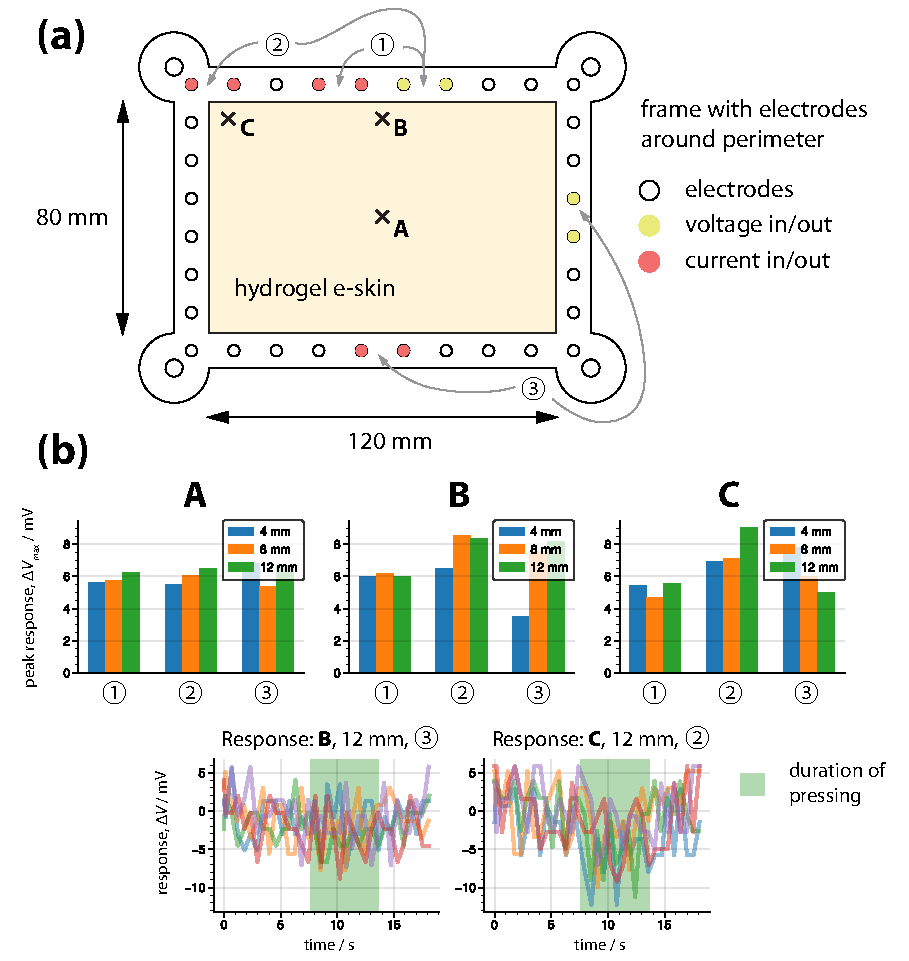
\includegraphics[width=0.9\columnwidth]{Images/Figure_1_diagram.pdf}
  \caption{\textbf{(a)} Diagram of the EIT setup. 32 electrodes are positioned around the perimeter of the rectangular frame. Current is injected and drained through one adjacent electrode pair and voltage is measured between another adjacent pair. The responses for three such electrode combinations are sampled for demonstration, labelled {\textcircled{\raisebox{-.9pt} {1}}}, {\textcircled{\raisebox{-.9pt} {2}}} and {\textcircled{\raisebox{-.9pt} {3}}}, with single-touch pressing points at sites \textbf{A}, \textbf{B} and \textbf{C} as shown. \textbf{(b)} The top row shows the maximum deviation in voltage response in the duration of pressing from the time-averaged unpressed baseline, for each press site, electrode combination, and press depth into the e-skin. In most cases, response increases with press depth, supporting the idea that the hydrogel's strain is responsible for its impedance changes. The bottom row shows the time-varying signal for five repeated trials of two selected cases: the response for (\textbf{C}, \raisebox{.5pt}{\textcircled{\raisebox{-.9pt} {2}}}) is clearer than for (\textbf{B}, \raisebox{.5pt}{\textcircled{\raisebox{-.9pt} {3}}}), the latter of which shows no distinguishable signal from the noise. This is likely because the press site is much further from the selected electrodes, so the displacement has no effect on the local impedance of the e-skin. The results in the top row for these cases are taken from the last of the five trials. To reduce the noise, the microcontroller collecting the EIT data applied an average over five samples at each time step, although considerable noise remained in our data even after this smoothing.}
  \label{fig:intro}
\end{figure}

Gelatin-based hydrogels are being increasingly used in soft robotic applications, demonstrating highly desirable flexibility, stretchability, environmental sensitivity, healability, tunability, and printability \cite{Heiden2022, Hardman2022, baumgartner2020resilient}. However, these additional functionalities, coupled with the nonlinearities of EIT's inverse problem \cite{Khan2019, Santosa1990}, causes difficulties in their analytic reconstructions from EIT hardware \cite{hardman2023tactile}. Their customisability for complex shapes and patterned sensors makes them a promising candidate for testing real-world data collection and training, requiring varied data from multiple touch locations.

In this work we explore the data-driven multi-touch responsivity of a functional gelatin-glycerol hydrogel e-skin, presenting two automated probing devices which can straightforwardly collect data from multiple points. We also investigate the effect of adding a conductive pattern to the surface of the hydrogel on the ability to predict touch location based on the EIT data using machine learning methods. Since this approach allows us to collect a much larger physical multi-point dataset than anything existing in the EIT-based e-skin literature, we end by discussing its implications for the validation and benchmarking of future developments.

% References for methods description
% \cite{Zhu2021EIT} % citation for fast EIT board we are using
% \cite{Adler_2006} % citation for EIDORS (analytic reconstructions)

\section{MATERIALS \& METHODS}
A sketch of the EIT frame containing 32 equally spaced M4 holes and four M6 holes at each corner was developed in Autodesk Fusion 360 and fabricated in PLA with a laser cutter. M4 screws were placed into these holes and bolted to the frame, after which an identical copy of the frame was placed on top for additional structural support.

The gelatin hydrogel was formed by mixing gelatin (pork, 240 bloom, MM Ingredients), glycerol (Fisher Scientific), water (not distilled), citric acid monohydrate (Fisher Scientific) and salt (NaCl) in ratios 1 : 1.5 : 2.5 : 0.2 : 0.1 by weight respectively. The mixture was stirred and incubated in a water bath at 50 $^{\circ}$C for two hours before pouring into a pre-made rectangular plastic container to a uniform depth of 5 mm. The internal dimensions of the container were 180 mm $ \times $ 120 mm, while the dimensions of the frame were 120 mm $ \times $ 80 mm, to allow the hydrogel to remain larger than the frame after contracting during cooling.

To construct the EIT setup, thick silicone (EcoFlex 10) supports were made and the freshly prepared hydrogel was placed on top, supported at the edges by a 3D printed plastic frame of identical cross-section to the ones described above. Four M6 screws were placed at the corners to fix these frames together, and the 32 screwheads were pushed into contact with the hydrogel to act as electrodes. All electrodes were connected to a microcontroller running the EIT program.

To gather data, a UR5 robot arm was fitted with a 3D printed gear and track connected to a servo motor powered by an Arduino. The robot was programmed to move the pressing tool to a given coordinate in the frame, push down, use the EIT microcontroller to measure impedances, before exiting the pressing motion. A 'deadzone' of 10 mm around the internal perimeter of the frame was enforced to avoid potential collisions between the robot and the hard plastic frame. For multi-touch applications, servos were attached to each finger and the press state could be programmed using a binary string, with 1 representing a finger down and 0 representing a finger up. All microcontroller programming was done in C++, using the PlatformIO environment in Visual Studio Code. All other programming was done in Python, using TensorFlow/Keras with Jupyter Notebooks for machine learning and serial communications for robot and Arduino interfacing.

An identical robot and plastic finger setup was used for all trials. Considerable noise from the EIT data was seen in all measurements, making analytic reconstruction challenging. During preliminary testing, it was observed that using one's real finger to press the skin produced far larger signals than those of to the plastic fingers, presumably due to the presence of the natural conductive oils (sebum) on the surface of the fingers. However, as the purpose of this study was to investigate the use of EIT based on material strain rather than the effects of exogeneous substances, usage of real fingers was not investigated further and the plastic fingers were used at all times.

\begin{figure}[htbp]
  \centering
  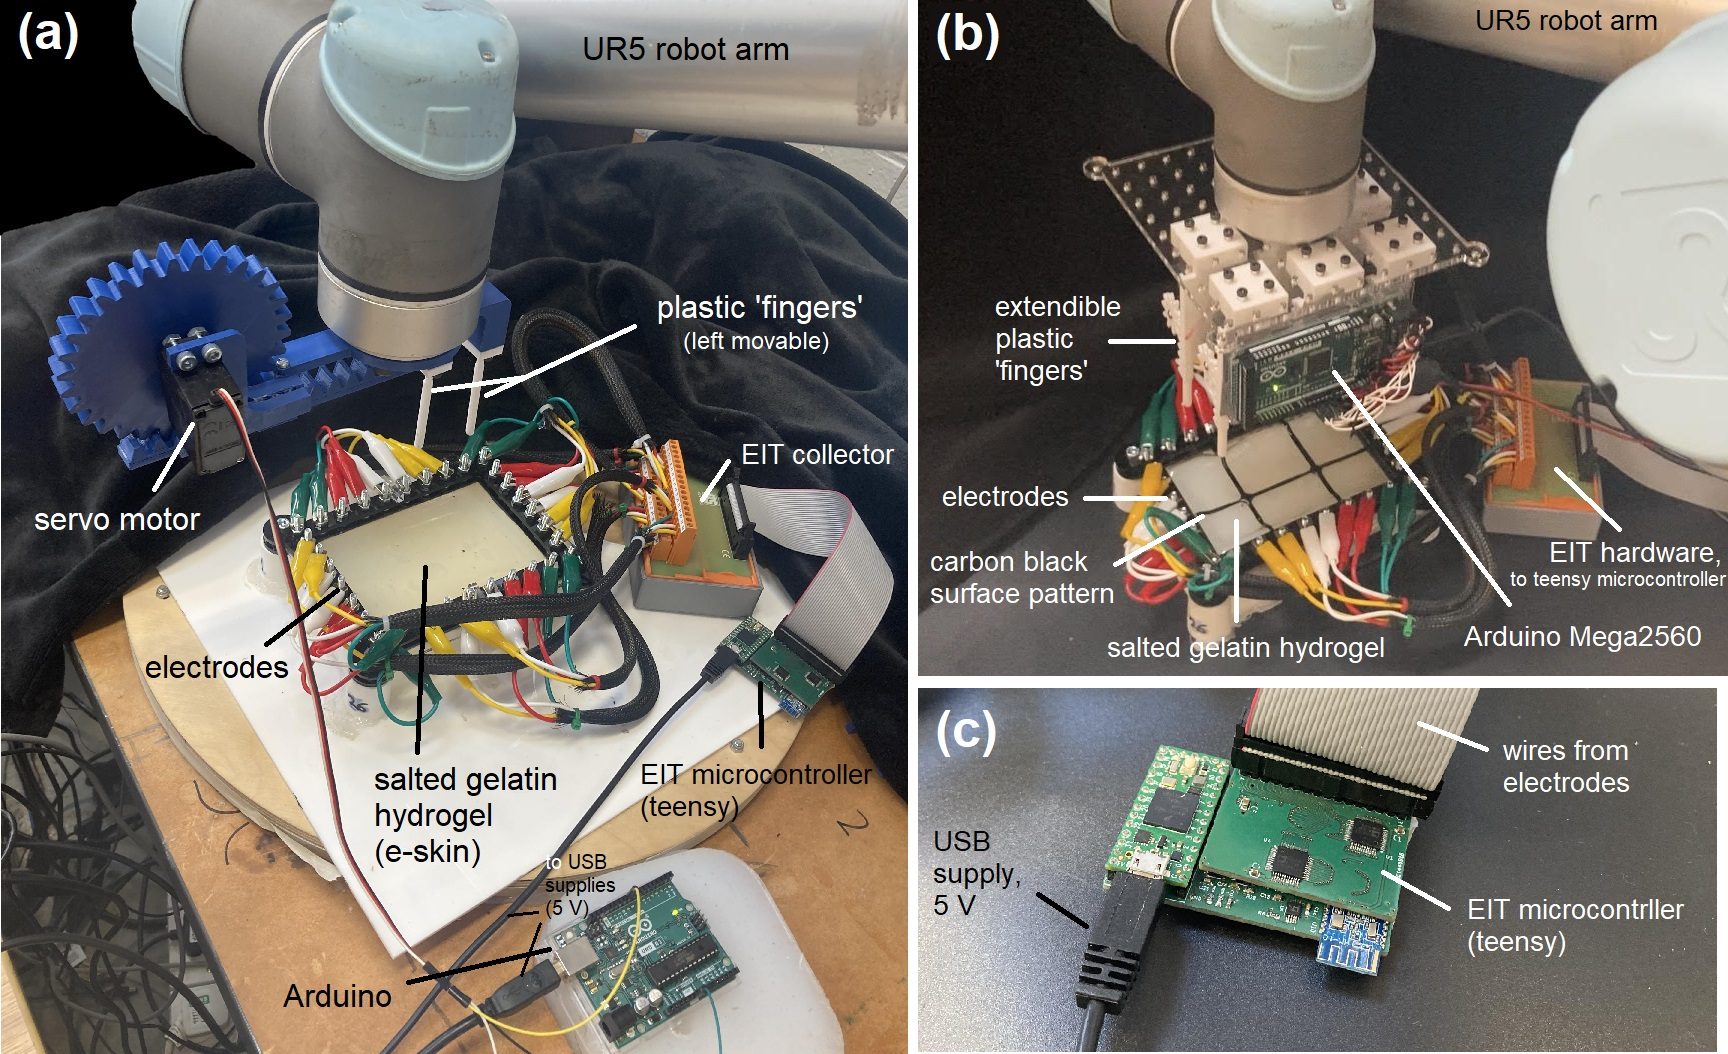
\includegraphics[width=0.9\columnwidth]{Images/Figure_2.jpg}
  \caption{\textbf{(a)} Setup for automatically collecting EIT touch data using two plastic fingers. The gear allows for variable distance between the fingers, while the robot allows for easily programmable translational and rotational motion. \textbf{(b)} Setup for collecting data with up to six retractable plastic fingers. This e-skin features an additional surface pattern of conductive carbon black in the shape of a $2 \times 3$ grid, which was found to improve the accuracy of multi-touch classification. \textbf{(c)} Close-up of the microcontroller used for carrying out the EIT experiments and sending the data to the PC via USB serial for analysis.}
  \label{fig:setup}
\end{figure}

\section{RESULTS \& DISCUSSION}

Data was collected initially for single points of touch, without any time-averaging of the EIT samples. Using three e-skins - one with salt, one with carbon black patterns, and one with both salt and carbon black patterns - separate datasets were collected with the number of data points totalling 3200, 550 and 550 respectively. Three machine learning model architectures were trained on each dataset, including a ridge regression model, a fully-connected (FC) feedforward neural network, and a convolutional neural network (CNN) whose output was a $ 6 \times 8 $ discretised grid of possible touch positions. Cross-validation and hyperparameter optimisation was applied where relevant. A copy of the Jupyter Notebook used to carry out the analysis is provided in the supplementary materials.

Broadly, the regression model performed poorly while the FC network performed the best, although still with considerable noise. A representative sample of five randomly selected points from the testing datasets and their predictions are shown in Fig. 3.

\begin{figure}[htbp]
  \centering
  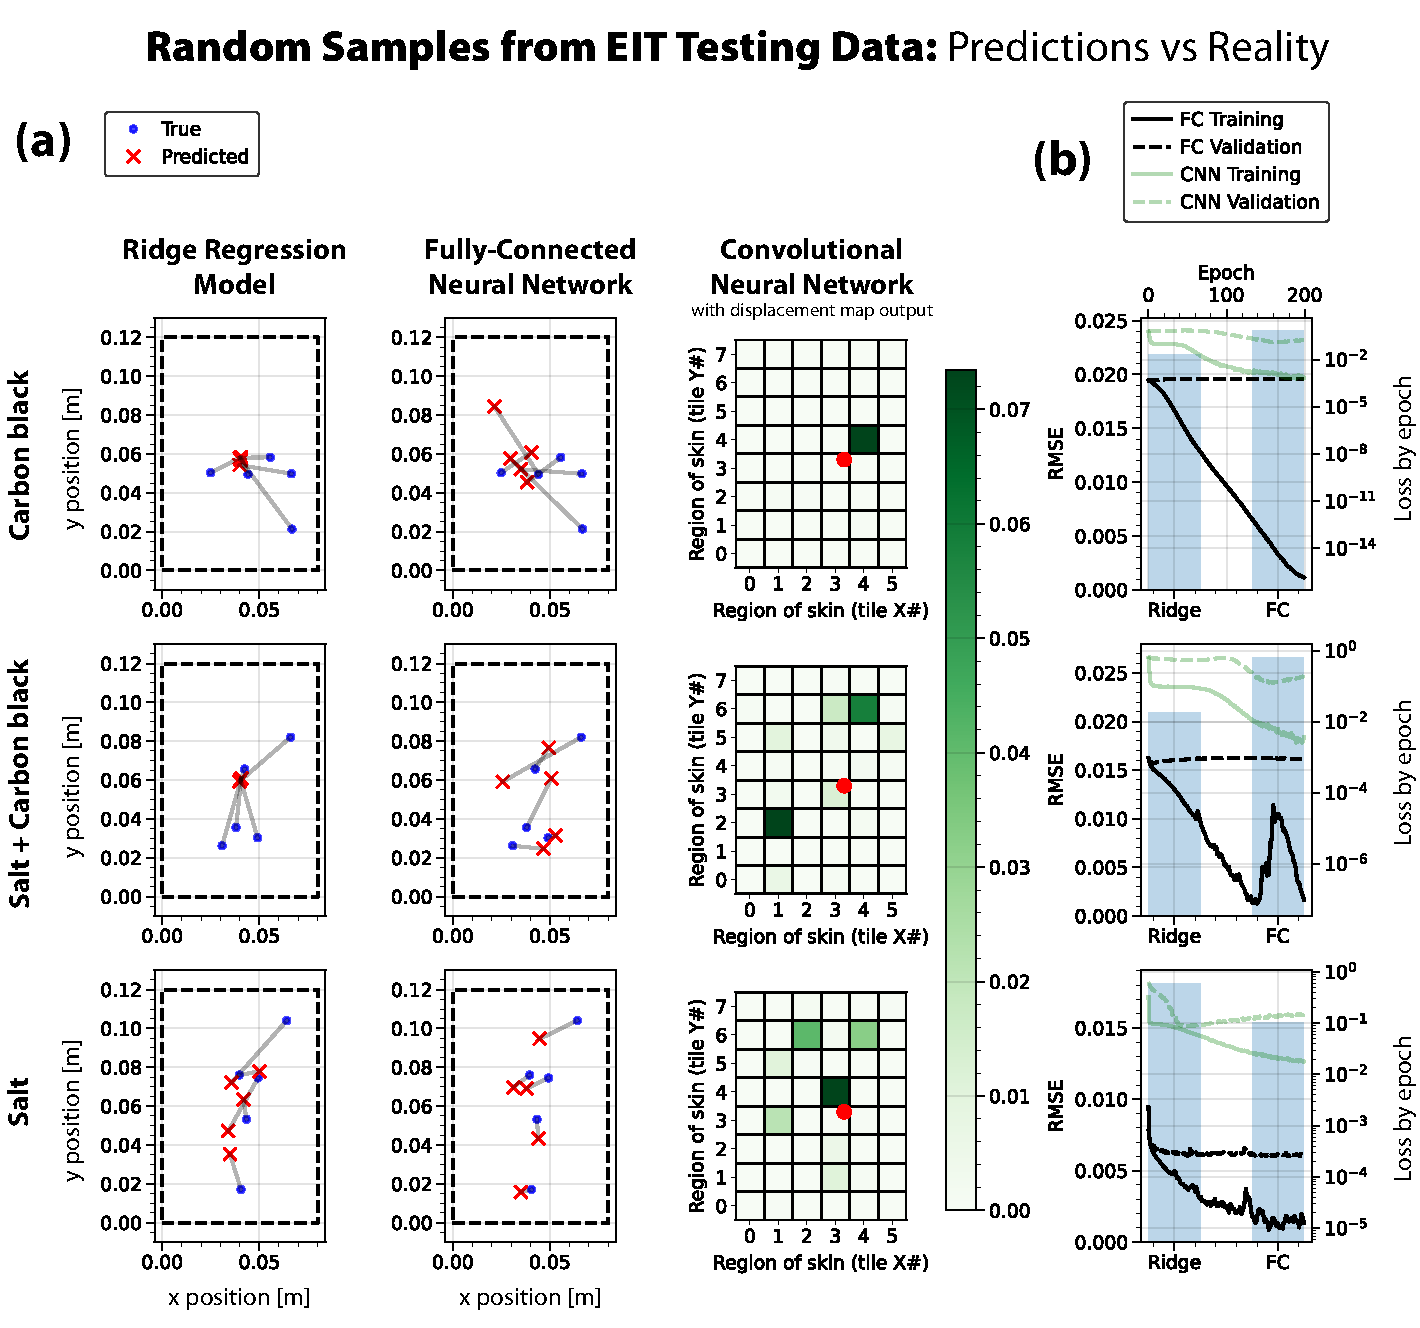
\includegraphics[width=0.9\columnwidth]{Images/Figure_3.pdf}
  \caption{\textbf{(a)} Single-touch predictions randomly sampled from the testing datasets for three different model architectures (ridge regression, feedforward neural network and convolutional neural network with a discretised output) for three different e-skins (with carbon black pattern, with salt and carbon black, with salt only). Five identical samples are shown for the regression and FC model on each skin, with one of these being shown for the CNN. The colourbar indicates the confidence score of the CNN on a given tile space on the skin. \textbf{(b)} The performance, as measured by root-mean-square-error (RMSE) of the ridge model and FC neural network are shown on the right column with bars for each skin (aligned with those in \textbf{(a)}), and the convergence of the training and validation losses of the FC neural network (mean square error) and the CNN (binary cross-entropy) are shown on the secondary axes.}
  \label{fig:proofofconcept}
\end{figure}

The six-finger dataset totalled $ N = 1100 $ data points, in which the touch 'position' (tile) was encoded as a 6-bit binary string. A convolutional neural network (CNN) was trained to map the standard-scaled, time-averaged EIT measurements $ \boldsymbol{x} \in \mathbb{R}^{1024} $ into the tile touch predictions $ \boldsymbol{y} \in \mathbb{R}^{6} $, where $ 0 \leq y_i \leq 1, \ \forall i \in \left \{  0 ... 5\right \} $. The datasets were split into 80:10:10 train-validation-test sets and trained with a mean-squared error (MSE) loss function.

Batch normalisation and pooling layers were included after each of the two convolutional layers in the network, with a final output layer having sigmoidal activation. Hyperparameter optimisation was used to minimise the validation loss after a fixed number of epochs.

\begin{figure}[htbp]
  \centering
  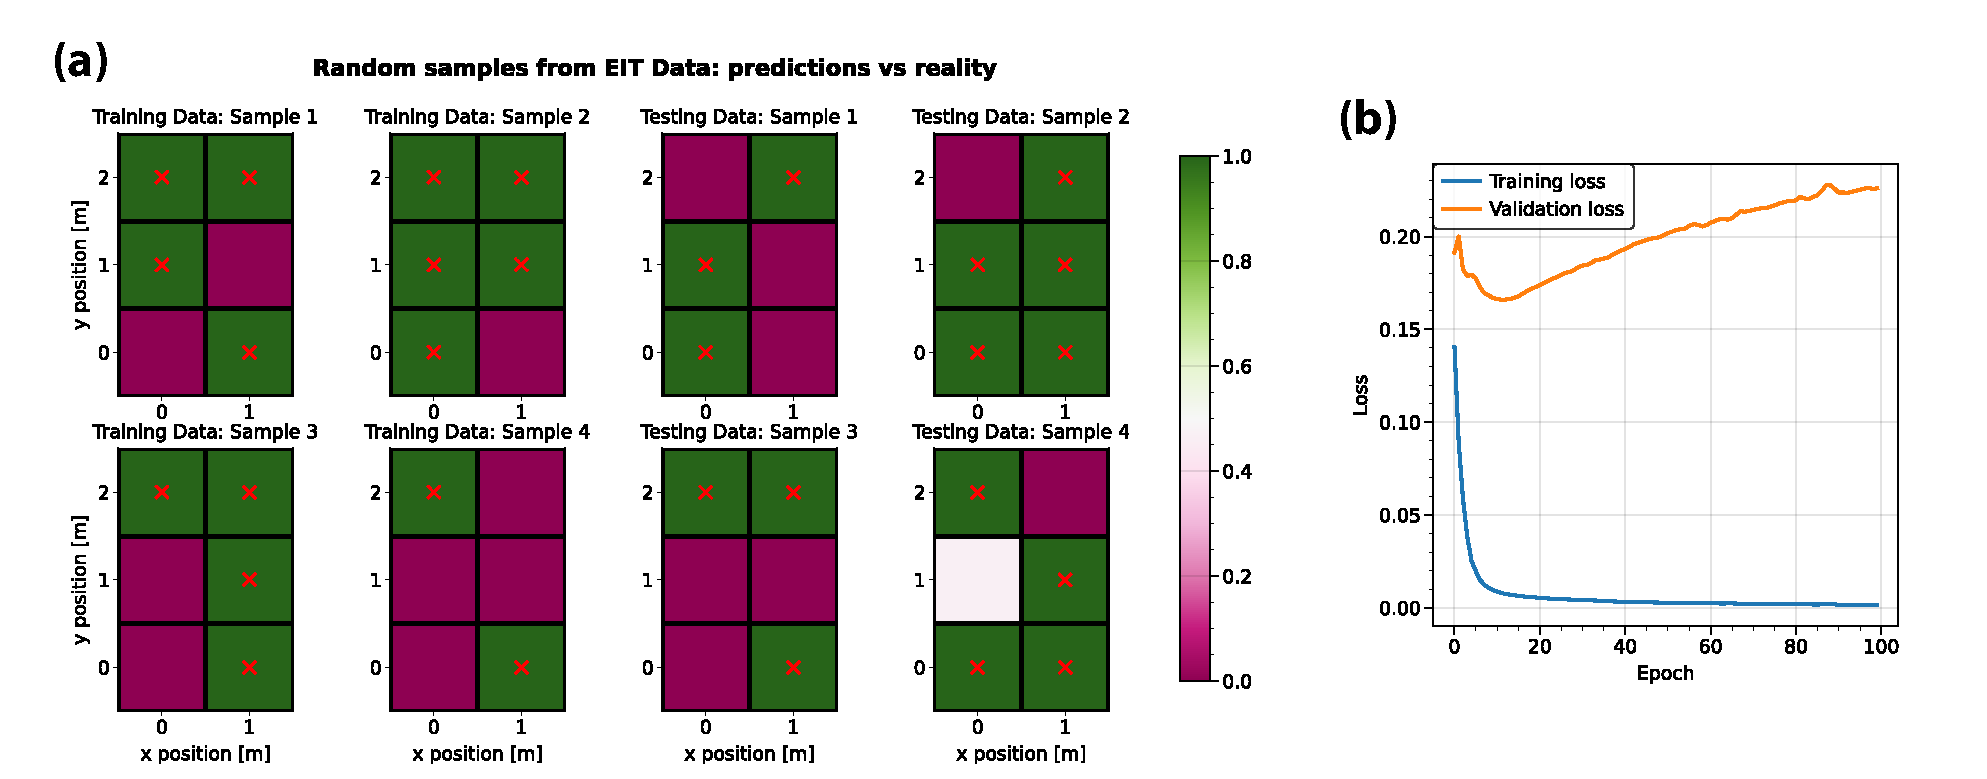
\includegraphics[width=0.9\columnwidth]{Images/Figure_4.pdf}
  \caption{\textbf{(a)} Randomly sampled data points featuring up to six points of touch in the training and testing sets. The red crosses $ {\textcolor{red}{\times}} $ are located at the centres of the six possible tiles and represent the actual tiles pressed. The ground truth pressing locations were programmed to vary randomly by up to $ \pm 8 $ mm in both $ x $ and $ y $ positions from these centre locations. Most predictions were correctly classified confidently as either pressed or unpressed; the 'near-white' tile in testing sample 4 is correctly classified as unpressed despite higher uncertainty. \textbf{(b)} Training and validation losses, as measured by the mean-squared error (MSE) of the network during training. It was found that validation loss began to increase after a larger number of epochs, potentially due to overfitting.}
  \label{fig:superposition}
\end{figure}

Applying a simple binary threshold (rounding to the nearest integer) to the output, the tiles being pressed were predicted. It was found that, the total proportion of correctly-identified tiles were 99.96\% and 97.58\% for the training and testing sets respectively. The total proportion of fully correct touch patterns (i.e. all six tiles were correctly labelled) were 99.77\% and 89.09\% for the training and testing sets respectively.

\begin{figure}[htbp]
  \centering
  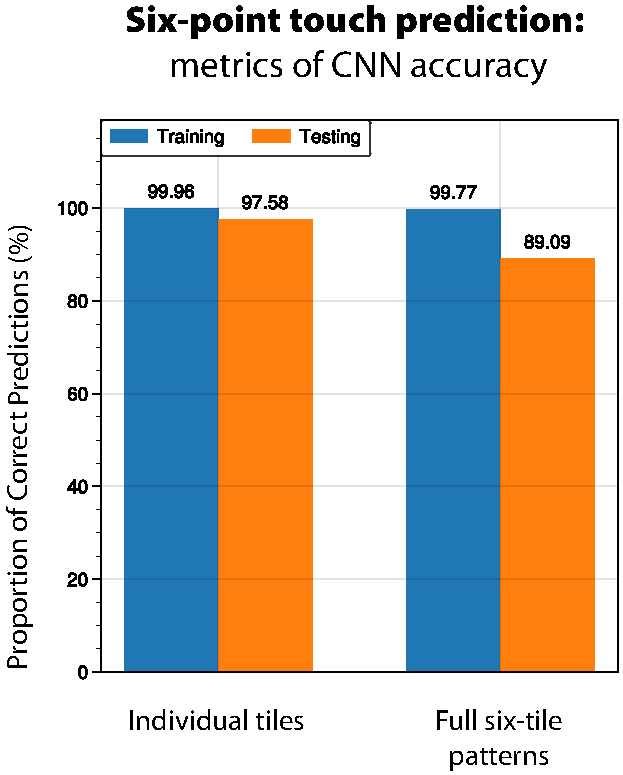
\includegraphics[width=0.9\columnwidth]{Images/Figure-5.pdf}
  \caption{Large 2-part figure: results of learning/regression approach, compared to generic analytic reconstruction. First part is qualitative: maps of predicted press locations for a select few examples. Second part backs up with data: average errors, spatial distribution of errors mapped etc. Results from this used to argue a few (say 3) patterns which might improve results in the worst-performing areas/cases.}
  \label{fig:processed}
\end{figure}

\begin{figure}[htbp]
  \centering
  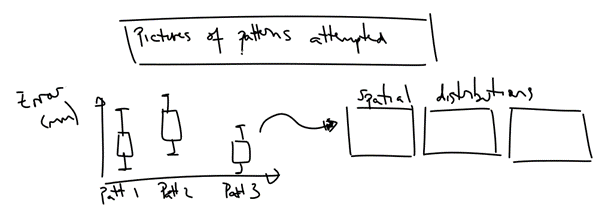
\includegraphics[width=0.9\columnwidth]{Images/filler4.png}
  \caption{Similar data for different patterns on the rectangular surface. Proof that these to different distributions of error/prediction, along with tensile test data to justify the mechanical coupling of the materials under strain.}
  \label{fig:patterns}
\end{figure}

\begin{figure}[htbp]
  \centering
  
\includegraphics[width=0.9\columnwidth]{Images/filler5.png}
  \caption{Additional data for the patterned samples, depending on the results we've obtained. Potentially demonstrating a trade-off between two parameters (such as better predictions for a fixed separation at the cost of worse predictions at smaller separations) - some kind of Pareto curve?}
  \label{fig:patternfollowup}
\end{figure}

\begin{figure}[htbp]
  \centering
  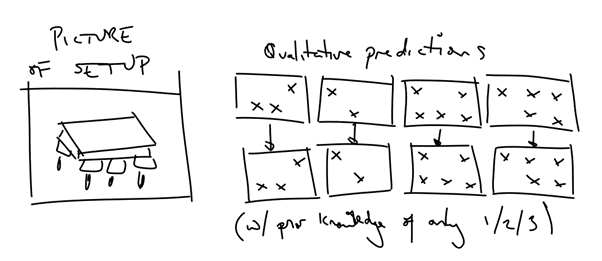
\includegraphics[width=0.9\columnwidth]{Images/filler6.png}
  \caption{Consolidating the main takeaways (patterns + learning approach) into one final demo. If we have trained our approach only with 1/2/3 probing points, can it be used to predict different combinations of the 6-probe presser? Excellent end to the paper if so.}
  \label{fig:finaldemo}
\end{figure}

\section{CONCLUSIONS}
Conclusion goes here.


% \addtolength{\textheight}{-12cm}   % This command serves to balance the column lengths
%                                   % on the last page of the document manually. It shortens
%                                   % the textheight of the last page by a suitable amount.
%                                   % This command does not take effect until the next page
%                                   % so it should come on the page before the last. Make
%                                   % sure that you do not shorten the textheight too much.

%%%%%%%%%%%%%%%%%%%%%%%%%%%%%%%%%%%%%%%%%%%%%%%%%%%%%%%%%%%%%%%%%%%%%%%%%%%%%%%%



%%%%%%%%%%%%%%%%%%%%%%%%%%%%%%%%%%%%%%%%%%%%%%%%%%%%%%%%%%%%%%%%%%%%%%%%%%%%%%%%



%%%%%%%%%%%%%%%%%%%%%%%%%%%%%%%%%%%%%%%%%%%%%%%%%%%%%%%%%%%%%%%%%%%%%%%%%%%%%%%%
% \section*{APPENDIX}

% Appendixes should appear before the acknowledgment.

\FloatBarrier

\section*{DATA AVAILABILITY}
Code is available on GitHub at the directory {\tt \href{https://github.com/lorcan2440/EIT\_Touch\_Sensor/blob/main/src/urop-data-analysis.ipynb}{https://github.com/lorcan2440/ \\ EIT\_Touch\_Sensor/blob/main/ \\ src/urop-data-analysis.ipynb}}.

\section*{ACKNOWLEDGMENT}
This work was supported by the Samsung Global Research Outreach Program (GRO G118293), and by by EPSRC DTP EP/R513180/1.

\section*{Author Disclosure Statement}
The authors declare no competing interests.

\bibliographystyle{ieeetr}
\bibliography{bibliography.bib}

\end{document}
